% Sort: 4 pages
% Full: 10 pages

\documentclass[conference]{IEEEtran}
\IEEEoverridecommandlockouts
% The preceding line is only needed to identify funding in the first footnote. If that is unneeded, please comment it out.
%Template version as of 6/27/2024

\usepackage{cite}
\usepackage{amsmath,amssymb,amsfonts}
\usepackage{algorithmic}
\usepackage{graphicx}
\usepackage{textcomp}
\usepackage{xcolor}
\def\BibTeX{{\rm B\kern-.05em{\sc i\kern-.025em b}\kern-.08em
    T\kern-.1667em\lower.7ex\hbox{E}\kern-.125emX}}
\begin{document}

\title{Linear Algebra Based Graph Analysis on RISC-V GPGPU Vortex
\thanks{Identify applicable funding agency here. If none, delete this.}
}

\author{\IEEEauthorblockN{1\textsuperscript{st} Given Name Surname}
\IEEEauthorblockA{\textit{dept. name of organization (of Aff.)} \\
\textit{name of organization (of Aff.)}\\
City, Country \\
email address or ORCID}
\and
\IEEEauthorblockN{2\textsuperscript{nd} Given Name Surname}
\IEEEauthorblockA{\textit{dept. name of organization (of Aff.)} \\
\textit{name of organization (of Aff.)}\\
City, Country \\
email address or ORCID}
\and
\IEEEauthorblockN{Semyon Grigorev}
\IEEEauthorblockA{\textit{dept. name of organization (of Aff.)} \\
\textit{name of organization (of Aff.)}\\
City, Country \\
email address or ORCID}
}

\maketitle

\begin{abstract}
Abstract!!!!
\end{abstract}

\begin{IEEEkeywords}
GraphBLAS, Sparse Linear Algebra, Graph Analysis, GPGPU, RISC-V
\end{IEEEkeywords}

\section{Introduction}

Context-Free Path Querying (CFPQ) is an actively developed area in graph database analysis.
CFPQ is also used for static code analysis~\cite{Reps,10.1145/193173.195287,Zheng}, RDF querying~\cite{10.1007/978-3-319-46523-4_38,MEDEIROS201975}, biological data analysis~\cite{cfpqBio}.

Most of research is focused on developping algorithms for CFPQ evaluation~\cite{hellingsRelational,ward2008distributed,cfpqBio,MEDEIROS201975,Azimov:2018:CPQ:3210259.3210264,Grigorev:2017:CPQ:3166094.3166104}, whereas specification languages for context-free queries are not investigated enough.
Best to our knowledge, only one extension for Sparql supports context-free constarints: cfSPARQL~\cite{10.1007/978-3-319-46523-4_38}.
There is also a proposal for CFPQ as a part of Cypher\footnote{Proposal with path pattern syntax for openCypher: \url{https://github.com/thobe/openCypher/blob/rpq/cip/1.accepted/CIP2017-02-06-Path-Patterns.adoc}.
It is shown that context-free constraints can be expressed with the proposed syntax. Access date: 30.03.2020} language, but there is no implementation for it yet.
We believe that more research should be conducted on the specification languages fo context-free constraints in graph querying.

It is worth noting that graph analysis is often only a part of a more complex system, usually implemented in a general-purpose language.
Since a graph query language is unsuitable to implement a whole system, there should be means of integration of them into general-purpose programming languages.
There are many ways to integrate them ranging from creating graph queries from string values of a general-purpose language to implementing a special embedded domain specific language, and even more sophisticated.

Although simple, the string manipulating approach does not provide a developper with any safety guarantees.
There is no way to ensure that a string generated by an application is a valid query or, in case it is not, to provide any feedback.
This makes string manipulating technique error prone, the code --- unclear and hard to maintain.

Safety of an embedded DSL entirely depends on its implementation.
Some general-purpose languages with powerfull type systems (such as \haskell{}, \ocaml{} or \scala{}) or the ones supporting hygienic macros (such as \scheme{} or \rust{}) facilitate creating safe and reliable DSLs.
Still, they typically lack full support of a development environment: it may be harder to debug queries or issues with composability may arise.

There is a general trend towards imposing more restricting type systems on programming languages.
Among many others are typing annotations for \python{} and \typescript{} code and nullability checks in \kotlin{}.
Typing graphs and query languages improves  readability and simplifies maintainance~\cite{10.1145/2076623.2076653}.

Parser combinators are the answer to the integration of parsing into a general-purpose programming language.
Recursive descend parsers are encoded as functions of the host language, while grammar constructions such as sequencing and choice are implemented as higher-order functions.
This idea was first introduced in~\cite{burge} and further developped in numerous works.
Notable development is monadic parser combinators~\cite{hutton1996monadic}.
In this approach, one can not only parse the input, but simultaneously run semantics calculation if parsing succeeds.
Paper~\cite{izmaylova2016practical} proposed the first monadic parser combinator library which solves the long-standing problem of inability to handle ambiguous and left-recursive grammars.
A library for graph querying was developped~\cite{10.1145/3241653.3241655} based on this work.
The core idea is to use generalized parser combinators as both a way to formulate a query and to execute it.
This approach inherits benefits of combinatory parsing: ease of code reuse, type safety guaranteed by the host language and, since the parser is simply a function, the integrated development support.

Besides integration, it can compute both the single-source and all pairs semantics, as well as execute user actions.
The~single-source semantics is relevant to many real-world applications, including manual data analysis.
It also may be less time-intensive, since on average it needs to expore only a subgraph of the input graph.
Many querying algorithms are only capable to compute all pairs reachability which makes them unsuitable for some applications.

In this paper we make the following contributions.
\begin{itemize}
  \item We demonstrate how to use combinatory-based graph querying on example.
  \item We illustrate such features of the approach as type-safety, flexibility (composability and generics), IDE support and computing user-defined actions.
  \item We evaluate single-source context-free path querying on some real-world RDFs.
  \begin{itemize}
    \item Based on our evaluation, the most common case in RDF context-free querying is when the number of paths in the answer set is big, but they are small.
    \item We demonstrate that the single-source CFPQ can feasibly be used to evaluate such queries.
    \item We conclude that there is a need for a further detailed analysis of both theoretical time and space complexity of single-source CFPQ.
  \end{itemize}
\end{itemize}

\section{Spla Graph Analysis Library}

Spla~\cite{spla} is a GPGPU‑accelerated, GraphBLAS‑inspired library for graph analysis.
It is based on sparse linear algebra and uses OpenCL to offload linear algebra kernels to appropriate devices, including GPGPUs.
Using OpenCL makes the library vendor-agnostic: it has been shown in~\cite{spla} that Spla performs and scales well across GPUs from different vendors including AMD, Intel, and Nvida.

The library implements several classical graph analysis algorithms, including canonical single-source level BFS, triangle counting (TC), single-source shortest path (SSSP), and PageRank.

\section{RISC-V GPGPU Vortex}

Vortex\footnote{\url{https://github.com/vortexgpgpu/vortex}}~\cite{10.1145/3466752.3480128} is an open-source RISC‑V‑based GPGPU.
It supports OpenCL programming via the POCL compiler\footnote{Portable Computing Language project: \url{https://portablecl.org/}}~\cite{10.1007/s10766-014-0320-y}.
Additionally, it is designed for FPGAs equipped with high-bandwidth memory (HBM), which is advantageous for graph processing.


The high-level architecture of the Vortex processor\footnote{Detailed architectural information is available at \url{https://github.com/vortexgpgpu/vortex/blob/master/docs/microarchitecture.md}.} is shown in Fig.~\ref{fig:vortex_arch}. 
The processor consists of \emph{clusters}, which may share an optional $L_3$ cache.
Each \emph{cluster} contains multiple \emph{sockets}, which may share an optional $L_2$ cache.
\emph{Sockets} consist of cores with shared $L_1$ cache, and each core hosts multiple threads.
Threads share local memory and are logically grouped into warps.

\begin{figure*}
    \begin{center}
        \includegraphics[width=0.8\textwidth]{pictures/Vortex_arch.pdf}
        \caption{Vortex architecture}
        \label{fig:vortex_arch}
    \end{center}
\end{figure*}

The design is flexibly configurable: the numbers of clusters, cores, threads, and warps in the target processor can be specified, and the $L_3$ and $L_2$ caches can be independently enabled or disabled.
Number of sockets calculated automatically such that socket size is a minimum of 4 and number of cores.

The Vortex design is distributed with SimX, a cycle-approximate functional simulator.
A cycle-accurate RTL simulation is also available.
Although the A extension (atomics instructions)\footnote{Supported RISC-V profiles are RV32IMAF and RV64IMAFD (\url{https://github.com/vortexgpgpu/vortex?tab=readme-ov-file\#specifications})} is declared, atomic operations are currently supported only in the SimX simulator and not in the RTL implementation.

\section{Evaluation}

The goal of this evaluation is to assess the performance scaling of Spla on Vortex.
Due to limitations in atomic operation support within the RTL implementation, all experiments were performed using the SimX functional simulator.

\subsection{Environment}

Initial testing revealed issues with floating-point operations, which produced incorrect results for some hardware configurations.
Consequently, we limited subsequent experiments to Breadth-First Search (BFS) and Triangle Counting (TC), excluding Single-Source Shortest Path (SSSP) and PageRank.
To keep simulation times manageable, we used a single graph from the SuiteSparse matrix collection\footnote{A diverse collection of sparse matrices from various domains: \url{http://sparse.tamu.edu/}}: soc-Epinions1, with 75~888 vertices and 508~837 edges.


We conducted two series of experiments.
The first varies the number of warps and threads per warp while keeping the number of clusters and cores fixed (at 2 and 4, respectively), with the goal of selecting the best core configuration while preserving multi-core execution to account for cache effects.
The second series, using the best configuration identified in the first step, varies the number of clusters and cores per cluster to assess scaling at the core and cluster levels.
Cache sizes were set to their default values: 16 KB for $L_1$, 1 MB for $L_2$, and 2 MB for $L_3$.

We use the number of cycles reported by SimX as a performance metric.
For multi-core configurations, we report the maximum cycle count across all cores.
During the experiments, we encountered unexpected behavior in SimX that led to out-of-memory exceptions. 
Therefore, some data points are missing from the graphs below.

\subsection{Results}

In figures~\ref{fig:tc_threads_warps} and~\ref{fig:bfs_threads_warps}

\begin{figure}
    \begin{center}
        \includegraphics[width=0.49\textwidth]{pictures/TC_threads_warps.pdf}
    \end{center}
    \caption{Scaling analysis of triangle counting for varying numbers of warps and threads per warp}
    \label{fig:tc_threads_warps}
\end{figure}

\begin{figure}
    \begin{center}
        \includegraphics[width=0.49\textwidth]{pictures/BFS_threads_warps.pdf}
    \end{center}
    \caption{Scaling analysis of BFS for varying numbers of warps and threads per warp}
    \label{fig:bfs_threads_warps}
\end{figure}

Best configuration for BFS is 2 warps, 8 threads per warp (16 threads total). 
Best configuration for TC is 4 warps, 16 threads per warp (64 threads total).


\begin{figure}
    \begin{center}
        \includegraphics[width=0.49\textwidth]{pictures/BFS_cores_clusters.pdf}
    \end{center}
    \caption{Scaling analysis of BFS for varying numbers of clusters and cores per cluster}
    \label{fig:bfs_cores_clusters}
\end{figure}


Edges per core on cycle. Compare with Spla on other GPUs.

\subsection{Scaling limitations analysis}

%sum(scoreboard stalls * lsu_percent) / sum(instr) * 100
To analyze the reasons for limited scaling as the number of threads increases, we measured the average utilization of the ALU and LSU, in terms of stall cycles, for the best BFS configuration.
The results are presented in Fig.~\ref{fig:bfs_alu_stalls} and Fig.~\ref{fig:bfs_lsu_stalls}, respectively.
The data indicate that the LSU is the performance bottleneck within the core.

The same bottleneck was observed in the scaling analysis across clusters and cores.
Whether increasing cache sizes can alleviate this problem remains a question for future research.
We anticipate that careful cache size tuning may help identify a more efficient configuration.

\begin{figure}
    \begin{center}
        \includegraphics[width=0.49\textwidth]{pictures/BFS_alu.pdf}
    \end{center}
    \caption{ALU stalls on BFS for the best configuration}
    \label{fig:bfs_alu_stalls}
\end{figure}

\begin{figure}
    \begin{center}
        \includegraphics[width=0.49\textwidth]{pictures/BFS_lsu.pdf}
    \end{center}
    \caption{LSU stalls on BFS for the best configuration}
    \label{fig:bfs_lsu_stalls}
\end{figure}
\section{Conclusion and Future Work}

Platform presented.

Education. Metaprogramming, translators development, GPGPU programming, etc.

Graph parsing.

Geterogenious porgramming generalization. Hopac is better then MBP~\footnote{\url{https://vasily-kirichenko.github.io/fsharpblog/actors}}.

Research: Automatic memory management.

Data to code translation (automata can be translated into code instead of data structures in memory)

Other technical improvements: IDE support, type provider improvements, new OpenCL standard support, runtime extension, etc.

\bibliographystyle{IEEEtran}
\bibliography{SplaOnVortex}

\end{document}
